\documentclass[a4paper,12pt]{article}

\usepackage[utf8]{inputenc}
\usepackage[style=authoryear,backend=biber]{biblatex}
\usepackage[a4paper, margin=2.5cm]{geometry}

\usepackage{amsmath}
\usepackage{amsfonts}
\usepackage{amssymb}
\usepackage{graphicx}
\usepackage{wrapfig}
\usepackage{wasysym}
\usepackage{float}
\usepackage{pgfplots}

%\usepgfplotslibrary{external}
%\tikzexternalize
\graphicspath{ {./images/} }

\renewcommand{\baselinestretch}{2}
\pgfplotsset{compat=1.18}
\renewcommand*\contentsname{Table Of Contents}

\addbibresource{bibliography.bib}

\newcommand{\ResearchQ}{To what extent does changing the length of a circular cantilever beam affect its resonant frequency, and how well can the theoretical model predict this relationship?}


\begin{document}

\begin{titlepage}
    \begin{center}
        \vspace*{1cm}

        \textbf{Investigating Factors Affecting the Resonant Frequency of Cantilever Beams}\\

        \vspace{.5cm}
        \textbf{Research Question:}
        \ResearchQ

        \vspace{0.5cm}
        International Baccalaureate Physics Extended Essay

        \vfill

        \vspace{0.8cm}

        Word Count:3194


    \end{center}
\end{titlepage}
\pagenumbering{Roman}
% Table of Contents
\tableofcontents
\addcontentsline{toc}{section}{Table Of Contents}
\pagebreak


\pagenumbering{arabic}

\section{Introduction}\label{Intro}%500rq have 211, maybe 250 more?

Cantilever beams, seemingly simple elements used in construction where one end of a beam is solidly attached and the other loose, has played a major role in engineering, historically,these structures were used for purely mechanical structures, such as buildings, cranes, balconies and bridges.\autocite{BuildingConstructionBook}\\
While the use of such simple elements is still common in traditional construction, their range of use expands far beyond macroscopic architecture, Nowadays cutting edge technology such as MEMS(micro-electromechanical) systems which integrate mechanical systems with electronics in a microscopic level, use such structures as well, such as microscopic cantilever beams are that are used as inertial sensors in gyroscopes to sense the tiny acceleration forces in various circumstances.\autocite{MemsBook}%Analysis and Design Principles of MEMS Devices

I was fascinated to learn that such simple structures lie at the core of technologies we take for granted today. This pushed me to further investigate their functionality and their dynamic properties. My research question is ``\ResearchQ'' and
I aim to determine how the length of the beam and the initial energy loaded into the beam will affect the frequency that the beam naturally vibrates at when excited using pure mathematics and Experimentally.
In addition to proving it mathematically and experimentally, I also intend to conduct a virtual experiment, using finite element analysis.
As shown in \eqref{eqn:theory}, I am expecting to see the frequency is inversely proportional to the square of its length, and to see no meaningful relationship between the frequency and the initial energy load.
\begin{align}%eqn:theory
\label{eqn:theory}
\begin{split}
f_{n}\propto \frac{1}{l^{2}}
\\
f_{n}\not\sim E_{initial}
\end{split}
\end{align}
I intend to derive the hypothesis \eqref{eqn:theory} in Section \ref{Theory} and show it to be true in Section \ref{FEA} and Section \ref{Experiment} Using computational dynamics and an experiment respectively, and discuss the results, potential errors in methodology and what could be improved in Section \ref{ResultsAnalysis}.

\section{Background Information}%745rn
    \subsection{Euler–Bernoulli Beam Theory}\label{BeamTheory}%203
    To analyze bending of thin beams with axial loads, the Euler–Bernoulli Beam Theory, also known as classic beam theory is commonly used.
    This theory, forming the basis of a lot of engineering formulae. This theory assumes the beam deformation comes mainly from the bending moment, with a negligible amount of shear deformation. The formula is generally expressed as a fourth order linear differential equation, allowing deflection to be calculated from applied load, flexural rigidity and the loads positioning on the beam. Solving this equation gives the deflection curve, enabling the calculation of stresses, shear forces and bending moments.\autocite{EngMechanics}
    There lie assumptions behind this theory, including isotropic(same in all directions) material behavior and uniform density which can be assumed true for high carbon steel such as the ones that are that are used in this experiment.\autocite{EngMechanics}
    As this theorem does not take shear deformation into account, the beam needs to be thin relative to its length so the shear forces become negligible, as such, the size of the beams have been specifically picked to avoid shear forces.
    As this theorem is only able to calculate static loads, we will further expand it on Section \ref{Theory} to derive the dynamic beam equation.

    \subsection{Finite Element Method}\label{FEM}%208rn, "done"
    In engineering, it is common to be faced with partial differential equations, these equations are usually complex and are computationally intense to calculate, for example, calculating heat transfer, fluid flow, or in the case of this paper, non-rigid bodies.
    The Finite Element Method(FEM) is a way method to estimate the result of the partial differential equation, by dividing the continuous space of the problem into smaller, discrete parts called finite elements.\\
    The collection of the finite elements is known as the mesh. By dividing the space, analysis within each element becomes simpler, and later combined to get an estimation, this allows the computation of the differential equations to be computationally simpler. As this is a method of estimation, the results are not always accurate, to get the estimate closer to reality, the mesh resolution is increased at the cost of compute time.\autocite{FEABook} \\
    The use of this method of engineering analysis is commonly known as Finite Element Analysis(FEA) and will be used as a virtual experiment in Section \ref{FEA} to simulate the cantilever beams natural frequency.
    As this method allows to simulate deformation of bodies, this tool is generally built into Computer Aided Design(CAD) suites and Onshape, a cloud based CAD suite will be used in this paper.\\
    \begin{figure}[H]
    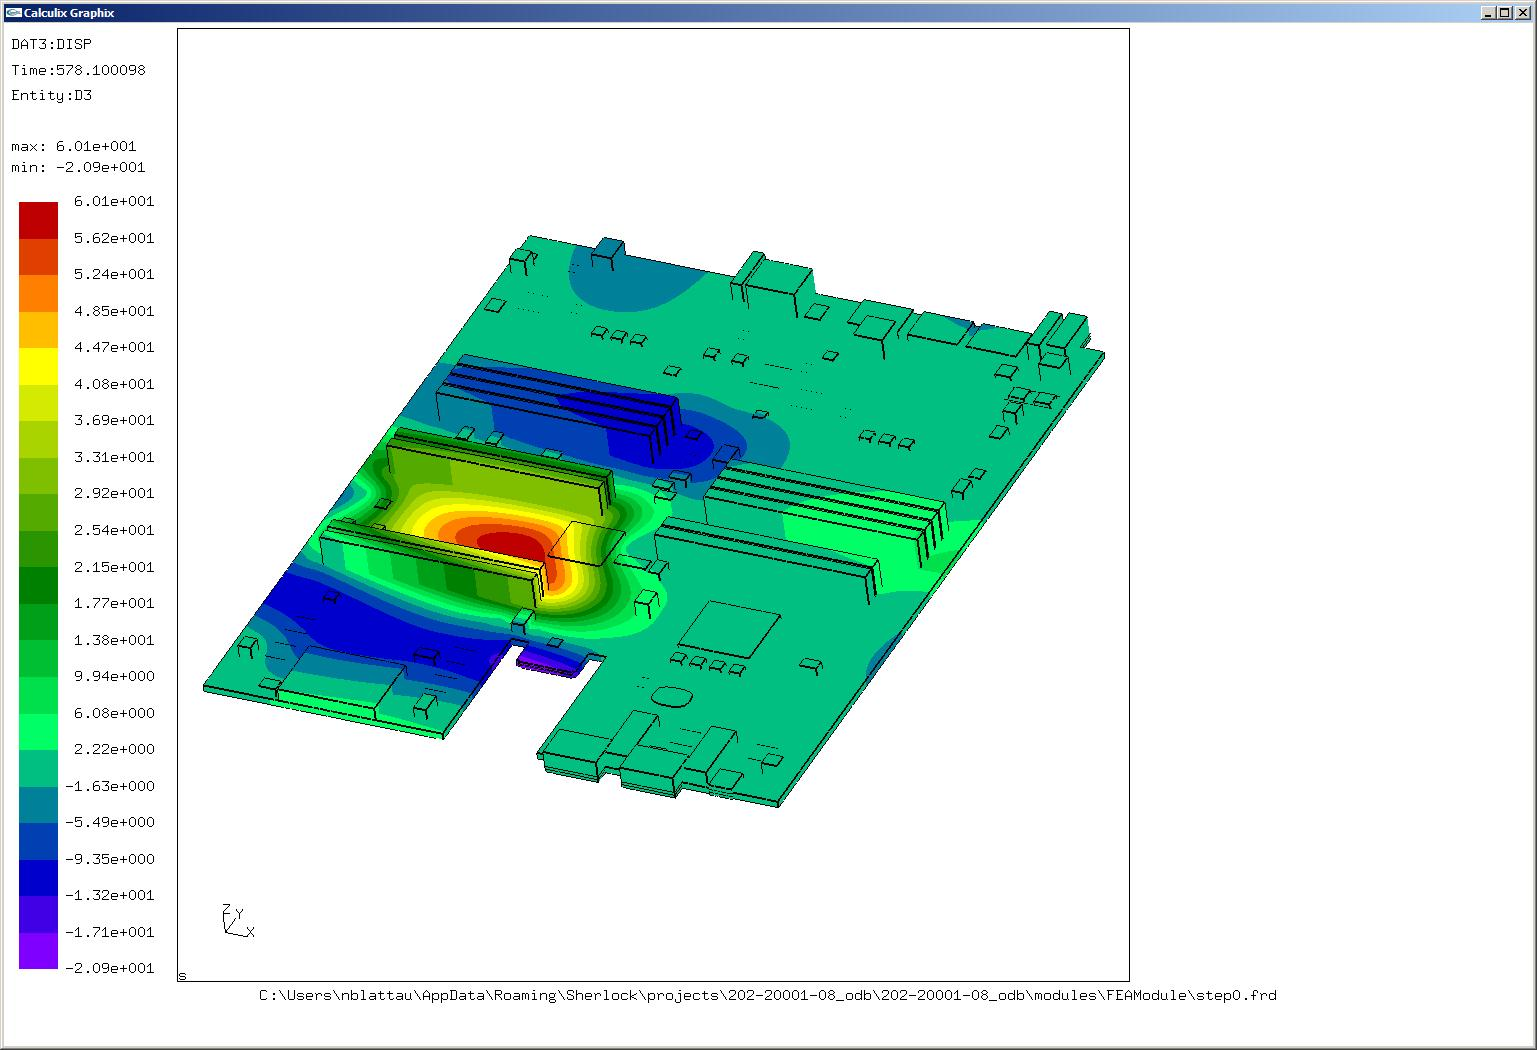
\includegraphics[width=0.6\textwidth]{feaexample}
    \centering
    \caption{The result of FEA\autocite{feaexample}}
    \centering
    \end{figure}

    \subsection{Fourier Transform} \label{FT}%332, done.
    The Fourier Transform(FT) is a fundamental mathematical technique used to break down time domain functions into their individual frequencies, essentially allowing to break a function down to its individual frequency components, indicating each frequencies amplitude and phase present in the original function.\\
    The mathematical principle behind the Fourier Transform is based on representing signals as a sum of cyclic functions, specifically sine and cosine.
    Any periodic signal is able to be represented as a sum of the sine and cosine functions, each with a unique amplitude and phase. This allows to break down a signal into its individual frequencies.
    In practice, continuous data sets cannot be attained, so the Discrete Fourier Transform is used. The Discrete Fourier Transform is the discrete counterpart of the traditional Fourier Transform, allowing it to work on finite data sets such as those attained in experimentation or communications.
    The Discrete Fourier Transform algorithm transforms a finite, equally spaced set of data in the time domain into a sequence of Discrete Fourier Transform coefficients, each representing the amplitude and frequency that when combined, makes up the signal.\\
    One of the major drawbacks of the Discrete Fourier Transform algorithm is its computational intensity, for that, the Fast Fourier Transform is used, the Fast Fourier Transform, instead of being a differential transform, is a computationally optimized recursive algorithm. Allowing for the Discrete Fourier Transform to of a signal to be calculated with much less compute power, this is especially useful for large data sets since the computational complexity of calculating the Discrete Fourier Transform is exponential with the datasets length.\autocite{FFTBook}

    For the specific purpose of analyzing a sound recording and breaking it down to its individual frequencies, the Fast Fourier Transform provides a direct and efficient way. By transforming the data formatted as pressure-time to the frequency domain, attaining frequency-amplitude data that allows us to see the dominant frequencies making up the signal, and this case, the dominant frequency will be the resonant frequency of the cantilever beam.

\section{Methodology} \label{Methodology}%none

    \subsection{Theory}\label{Theory}%500

    In Section \ref{BeamTheory},the static beam theory was introduced. Now, to determine the relationship for the resonant frequency of a cantilever beam, will be derived aiming to show its inverse square proportionality to length and independence from initial energy, as hypothesized in \eqref{eqn:theory}.

    Starting with the Static Beam Equation \eqref{eqn:SBeamTheory}:
    \begin{equation}\label{eqn:SBeamTheory_short}
    \frac{d^{2}}{dx^{2}}(EI\frac{d^{2}w}{dx^{2}})=q(x)
    \end{equation}
    To consider dynamics, the static load $q(x)$ is replaced with the inertial force per unit length, $-\rho A \frac{\partial^2 w(x,t)}{\partial t^2}$, leading to the Dynamic Beam Equation for unconstrained vibration:
    \begin{equation}\label{eqn:DBeamTheory_short}
    EI\frac{\partial^{4}w(x,t)}{\partial x^{4}} + \rho A \frac{\partial^2 w(x,t)}{\partial t^2} = 0
    \end{equation}
    assuming constant flexural rigidity $EI$.  For natural frequencies, harmonic motion is assumed as: $w(x,t) = W(x) \cos(\omega t)$. Substituting this into \eqref{eqn:DBeamTheory_short} and simplifying gives the spatial ordinary differential equation:
    \begin{equation}\label{eqn:SpatialODE_short}
    EI\frac{d^{4}W(x)}{d x^{4}} - \rho A \omega^2 W(x) = 0
    \end{equation}
    Letting $\beta^4 = \frac{\rho A \omega^2}{EI}$:
    \begin{equation}\label{eqn:SpatialODE_simple_short}
    \frac{d^{4}W(x)}{d x^{4}} - \beta^4 W(x) = 0
    \end{equation}
    For a cantilever beam, boundary conditions are: at the fixed end ($x=0$), $W(0) = 0$ and $W'(0) = 0$; at the free end ($x=l$), $W''(l) = 0$ and $W'''(l) = 0$. Solving this eigenvalue problem gives solutions for specific $\beta$ values, determining natural frequencies $\omega_n$.  For the fundamental mode, $\beta_1 l \approx 1.875$.

    Since $\beta^4 = \frac{\rho A \omega^2}{EI} = \frac{\rho A (2\pi f)^2}{EI}$, we have $\beta \propto \sqrt{f}$. Combined with $\beta_1 l \approx \text{constant}$, this leads to $\sqrt{f_1} l \approx \text{constant}$, and squaring both sides gives:
    \begin{equation}\label{eqn:frequency_length_inverse_square_short}
    f_1 \propto \frac{1}{l^2}
    \end{equation}
    This confirms the relationship between frequency $f$ and length. The proportionality constant depends on material ($E, \rho$) and geometry ($I, A$),and is kept constant in throughout the experiments.

    Regarding the second part of the hypothesis, frequency is a property of the system, determined by material and dimensions. Initial energy affects vibration amplitude, not frequency. The frequency is set by length. Thus, resonant frequency is theoretically independent of initial energy, supporting the hypothesis. $f_{n}\not\sim E_{initial}$. \autocite{EngMechanics}

    \subsection{Finite Element Analysis} \label{FEA}%338, donezo
    As explained in Section \ref{FEM}, FEA is a method to compute partial differential equations, and as shown in Section \ref{Theory} the resonant frequencies of the beam can be calculated with an partial differential equation.
    Thankfully, there exists tools to calculate the Finite Element Model built-in on many CAD suites to make the calculations, in this case, PTC's Onshape is to be used.\\
    To start, we need to define the variables and constants.
    \begin{align}%eqn:constants
    \label{eqn:constants}
    \begin{split}
    \diameter&=22mm
    \\
    l_{1}&=200mm\\
    l_{3}&=150mm\\
    l_{5}&=100mm\\
    E_{1}&=5\text{ J}\\
    E_{2}&=7.5\text{ J}\\
    E_{3}&=10\text{ J}\\
    \end{split}
    \end{align}
    As shown in \eqref{eqn:constants}, The diameter $\diameter$ and length $l$ have been picked according to commonly available materials and for ease of assess, the lengths picked should also be able to give a wide variety of frequencies.
    Additionally, the material properties of hardened carbon steel are required to run the simulation, shown in \eqref{eqn:steel}, these values were taken from Onshape.
    \begin{align}%eqn:steel
    \label{eqn:steel}
    \begin{split}
    \rho&=7.850\times10^{-6}~\frac{kg}{mm^{3}}\\
    \nu&=0.292\\
    E&=200000000000~Pa\\
    \end{split}
    \end{align}
    Where $\rho$ is the Density, $\nu$ is Poisson's ratio and $E$ is Young's Modulus
    \begin{figure}[H]%fig:VarTable
    \begin{center}
    \begin{tabular}[H]{|c||c|c|c|c|}
    \hline
    Variable & Length $l$ & Energy $E$ & Deformation $\epsilon$ & Frequency $f$ \\
    \hline\hline
    Type & Independent & Independent & Dependent & Dependent \\
    & Discrete & Discrete & Continuous & Continuous \\
    \hline
    Unit & mm & J & mm & hz, s$^{-1}$ \\
    \hline
    \end{tabular}
    \end{center}
    \caption{The Table Of Variables}\label{fig:VarTable}
    \end{figure}
    The Table of variables is as Figure \ref{fig:VarTable}, or in other words, length $l$ and energy $E$ will be changed according to \eqref{eqn:constants} and a separate simulation will be ran for each.
    \begin{figure}[H]%fig:CADPic
    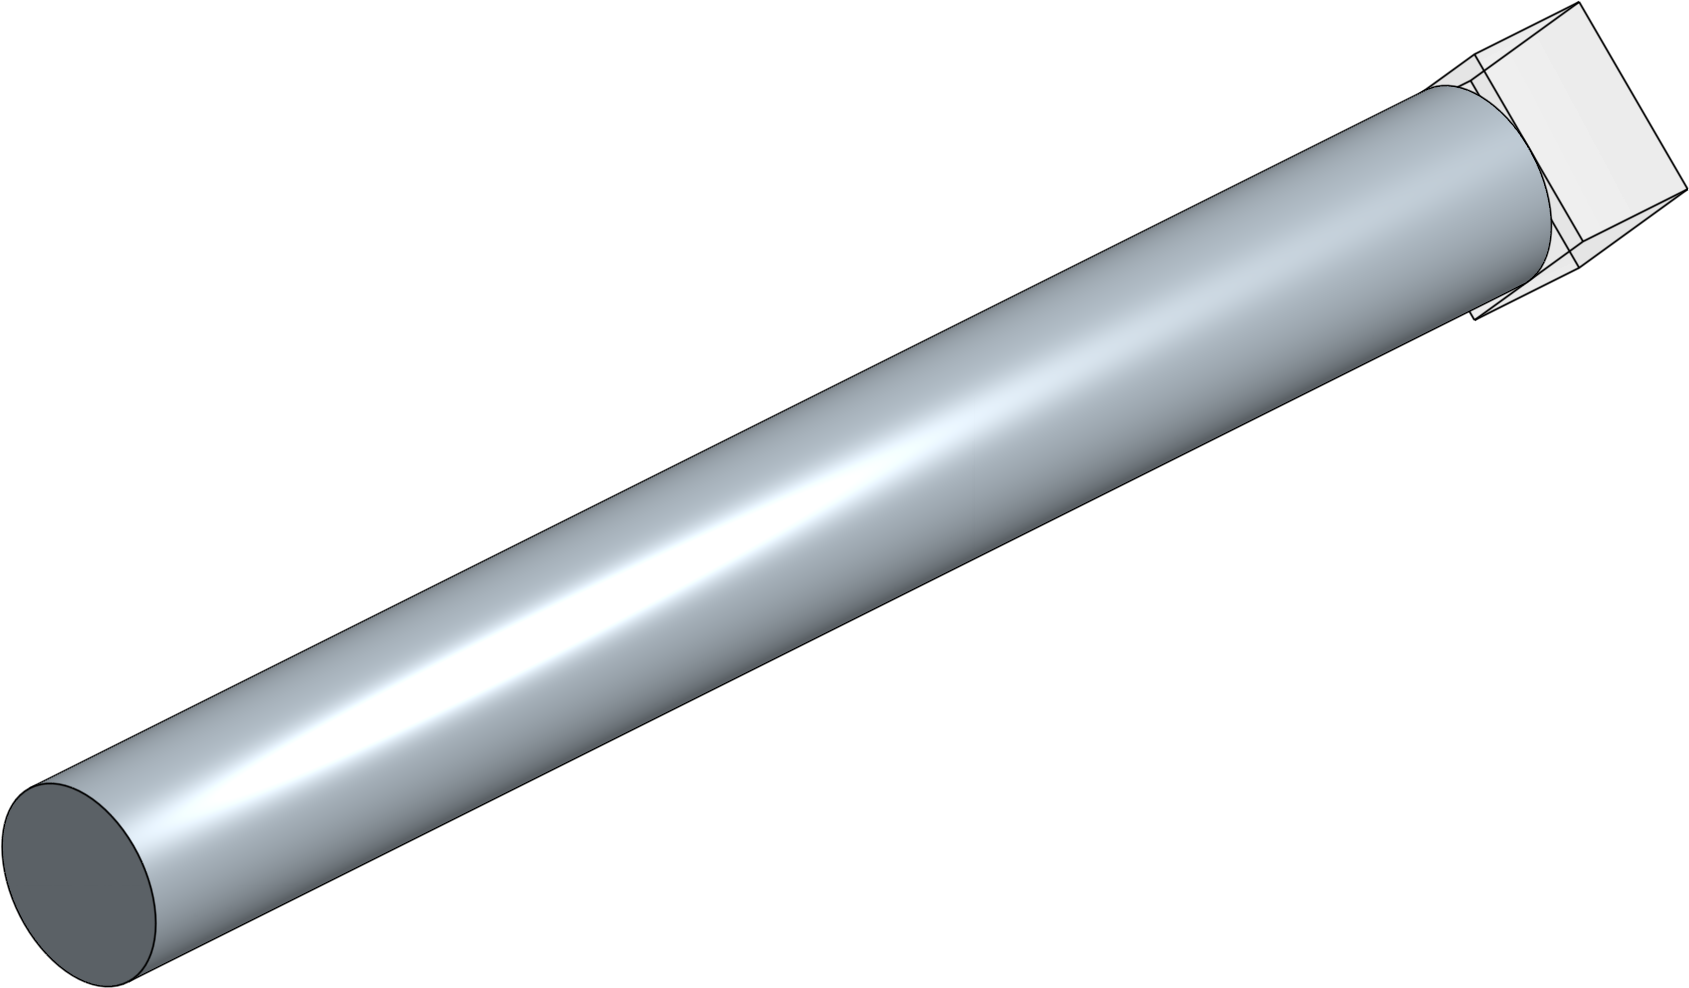
\includegraphics[width=0.5\textwidth]{CADPic}
    \centering
    \caption{The Design of the Circular beam, $\diameter=22mm$ and $l=200mm$}\label{fig:CADPic}
    \centering
    \end{figure}
    To start, a model was created for each length $l$, and was attached to a solid block as a reference frame. The 200mm long one can be seen in Figure \ref{fig:CADPic}
    And for each block, the Finite Element simulation was run 3 times, once per $E$ value.
    The deformation model for each model can be seen in Figure \ref{fig:FEAPic}, and the readings from the simulation was put into Figure \ref{fig:FEAtable} and as expected, initial energy $E$ shows no correlation with the frequency $f$, and the second part of \eqref{eqn:theory} has been shown true.
    \begin{figure}[H]%fig:FEAPic
    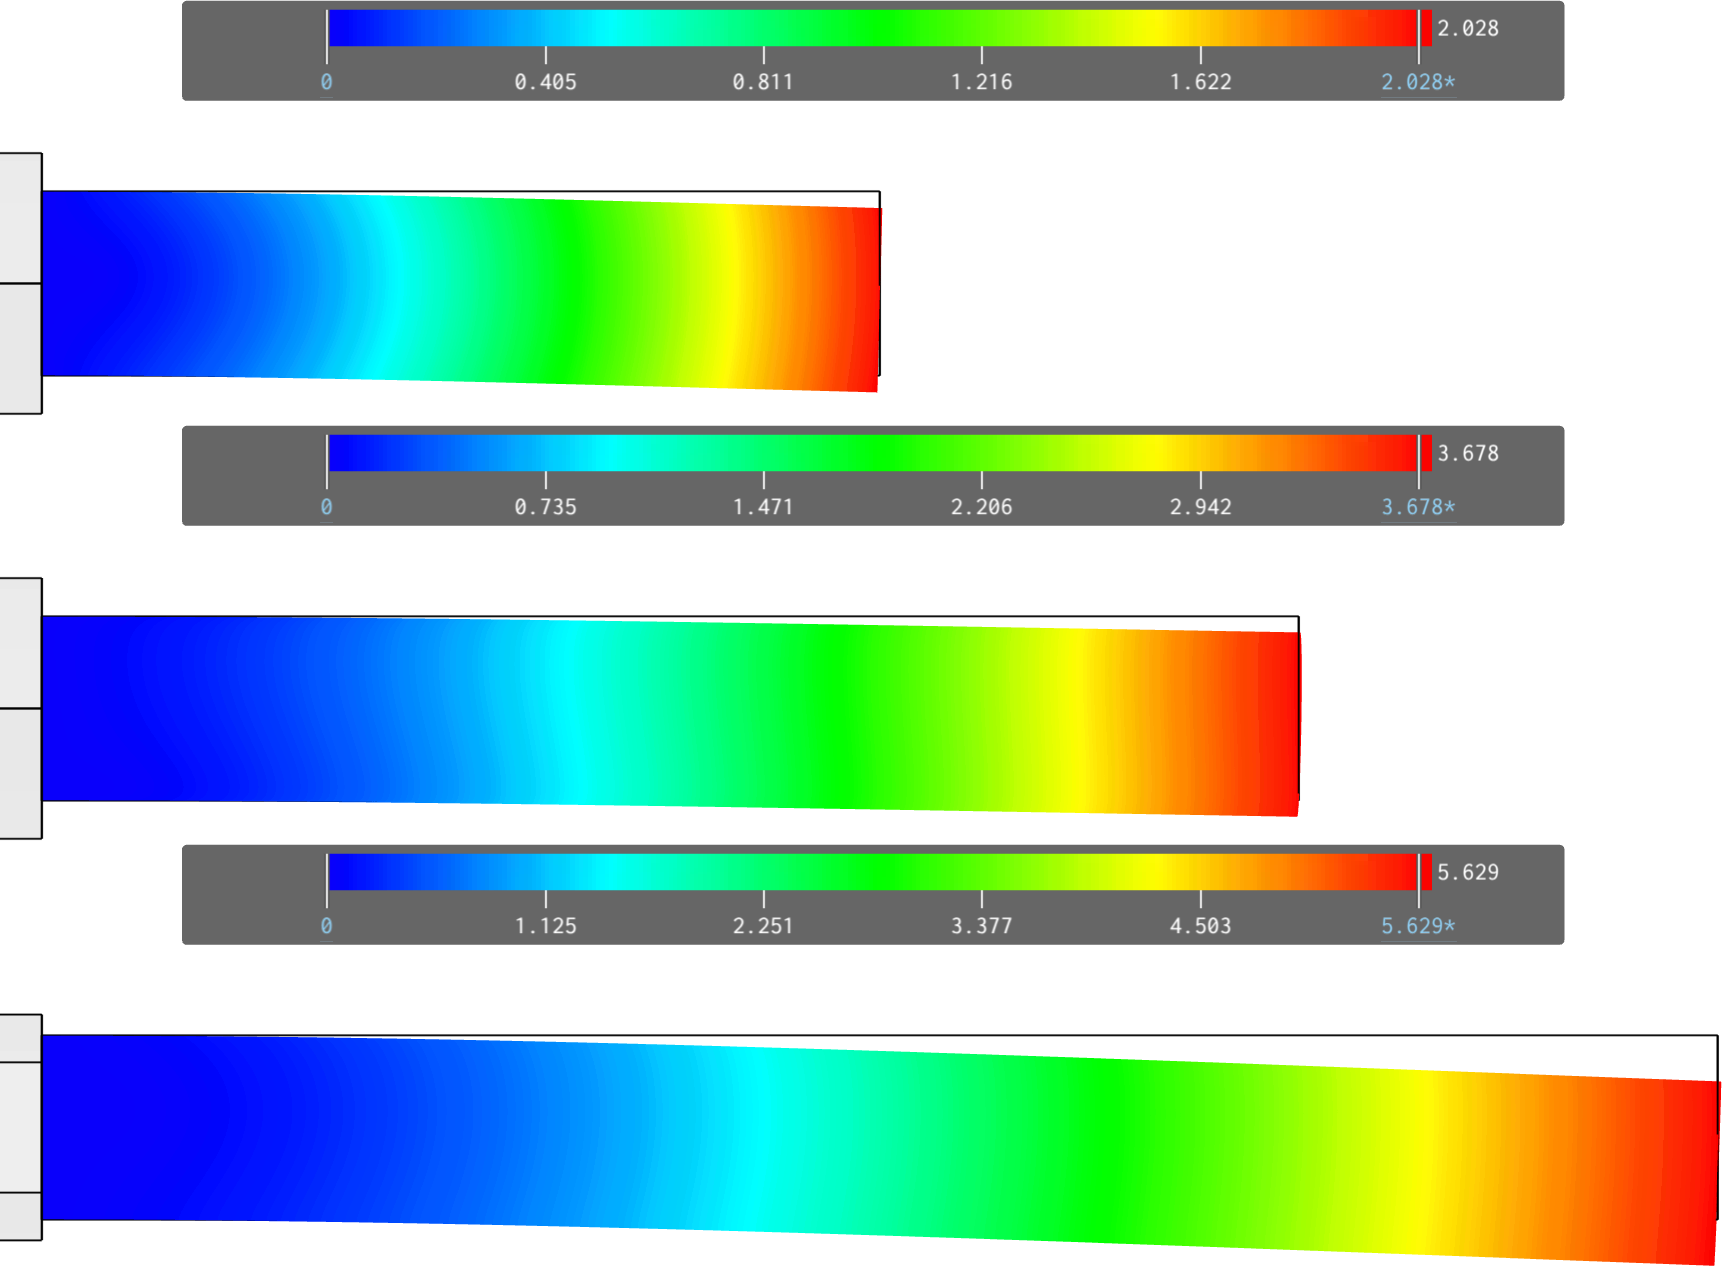
\includegraphics[width=0.7\textwidth]{FEA3}
    \centering
    \caption{The result of FEA, With the colors representing Deformation $\epsilon$ in mm.}\label{fig:FEAPic}
    \centering
    \end{figure}
    \begin{figure}[H]%fig:FEAtable
    \begin{center}
    \begin{tabular}[H]{|c|c||c|c||c|}
    \hline
    $l$ & $E$ & $f$ & $\epsilon$ & $\frac{1}{l^{2}}$\\
    \hline\hline
    100mm & 5 J & 1536 hz & 1.434 mm & $10^{-4}~mm^{-2}$\\
    \hline
    100mm & 7.5 J & 1536 hz & 1.756mm & $10^{-4}~mm^{-2}$ \\
    \hline
    100mm & 10 J & 1536 hz & 2.028mm & $10^{-4}~mm^{-2}$\\
    \hline
    150mm & 5 J & 694.2 hz & 2.601mm & $4.44\times10^{-5}mm^{-2}$\\
    \hline
    150mm & 7.5 J & 694.2 hz & 3.185mm & $4.44\times10^{-5}mm^{-2}$\\
    \hline
    150mm & 10 J & 694.2 hz & 3.678mm & $4.44\times10^{-5}mm^{-2}$\\
    \hline
    200mm & 5 J & 392.9 hz & 3.981mm & $2.5\times10^{-5}mm^{-2}$\\
    \hline
    200mm & 7.5 J & 392.9 hz & 4.876mm & $2.5\times10^{-5}mm^{-2}$\\
    \hline
    200mm & 10 J & 392.9 hz & 5.630mm & $2.5\times10^{-5}mm^{-2}$\\
    \hline
    \end{tabular}
    \end{center}
    \caption{The FEA Results}\label{fig:FEAtable}
    \end{figure}
    For the first part of \eqref{eqn:theory}, the modeling of $\frac{1}{l^{2}}$ in relation to $f$ is required, so for each value of $l$, and calculating it for each of gives the $\frac{1}{l^{2}}$ column of Figure \ref{fig:FEAtable} and the unit analysis regarding the unit of $\frac{1}{l^{2}}$ is given in \eqref{eqn:unitconv}.
    \begin{align}%eqn:unitconv
    \label{eqn:unitconv}
    \begin{split}
    \text{Given:}\\
    l&=\text{mm}\\
    f^{2}&=\text{mm}^{2}\\
    \text{Thus:}\\
    \frac{1}{f^{2}}&=\text{mm}^{-2}\\
    \end{split}
    \end{align}
    According to \eqref{eqn:theory}, $\frac{1}{l^{2}}$ and $f$ should be proportional, in other words, when graphed, the best line of fit should be a straight line crossing the origin, or in mathematical terms, $f \approx k \frac{1}{l^{2}}$ where $k$ is arbitrary.
    Doing the regression analysis, using ``LibreOffice Calc'', we get $f=15226342\frac{1}{l^{2}}+13.9$, or $f\propto\frac{1}{l^{2}}+9.1\times10^{-7}$ and the coefficient of determination is $R^{2}=0.99998$, showing strong correlation as seen in Figure \ref{fig:regression}\\
    While the result is off by $9.1\times10^{-7}$, this error is small enough in magnitude to be negligible.
    \begin{figure}[H]%fig:regression
    \begin{center}
    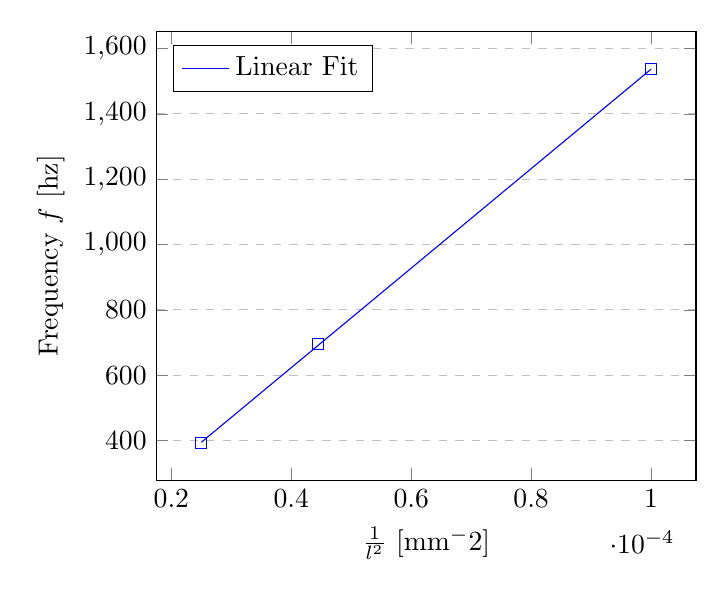
\begin{tikzpicture}
    \begin{axis}[
        xlabel={$\frac{1}{l^{2}}$ [mm$^-2$]},
        ylabel={Frequency $f$ [hz]},
        legend pos=north west,
        ymajorgrids=true,
        grid style=dashed,
    ]
    \addplot [
        domain=2.5e-5:1e-4,
        samples=100,
        color=blue,
        ]
        {15226342.949*x + 13.971};
    \addlegendentry{Linear Fit}
    \addplot+[
        only marks,
        color=blue,
        mark=square,
        ]
        coordinates {
        (1e-4,1536)(4.44e-5,694.2)(2.5e-5,392.9)
        };
    \end{axis}
    \end{tikzpicture}

    \caption{Table of ($\frac{1}{l^{2}}$,$f$) and linear regression}\label{fig:regression}
    \end{center}
    \end{figure}


    \subsection{Experiment}\label{Experiment}%500
    As shown in Section \ref{FEA}, the results of the Finite Element Analysis follow the expected relation in Section \ref{Theory}. And thus, this experiment aims to replicate the simulation setup used previously, and show that (a) The natural frequency values match those from Figure \ref{fig:FEAtable} and (b) the natural frequency follows the model as shown in equation \eqref{eqn:theory}.\\
    The material of the experiment is shown in Figure \ref{fig:materials}. And the initial energy loaded into the material will be controlled by the height of the hammer $h$ as given by the gravitational potential energy, as shown in \eqref{eqn:mgh}.
    \begin{figure}[H]%fig:materials
    \begin{equation}\label{eqn:mgh}
     E=mgh
    \end{equation}
    To calculate the energy of the hammer, $m=2\text{ kg}$ and $g=9.81\text{ms}^{-1}$ is substituted in \eqref{eqn:mgh} to get \eqref{eqn:hammerE}, additionally, the units of $h$ has been converted to meters.
    \begin{align}%eqn:hammerE
    \label{eqn:hammerE}
    \begin{split}
     E&=\frac{h}{1000}~9.81\times2\\
     E&=0.01962h \text{ J}
    \end{split}
    \end{align}

    \begin{center}
    \begin{tabular}[H]{|c|c|c|c|}
    \hline
    1 & 2 & 3 & 4\\
    \hline
    Metal Bar & Hammer & Vise & Sound Recorder\\
    \hline
    \end{tabular}
    \end{center}
    \caption{The Materials Used in The Experiment}\label{fig:materials}
    \end{figure}
    The Table Of variables as seen in  Figure \ref{fig:ExpVarTable} is similar to Figure \ref{fig:VarTable}  found in Section \ref{FEA} but a few changes were made to facilitate the experiment, notably, the deformation of the material $\epsilon$ is no longer measured, because of the difficulty that arises from trying to measure it while leaving frequency $f$ unaffected. And finally, hammer height has been added as a variable, this is the method for controlling the initial energy load $E$ for the analysis.\\
    The same values for $\diameter$, $l$ and $E$ will be used as \eqref{eqn:constants} in Section \ref{FEA}, the values for $h$ will be calculated according to \eqref{eqn:hammerE}, shown in \eqref{eqn:hvals}.

    \begin{align}%eqn:hvals
    \label{eqn:hvals}
    \begin{split}
     5 \text{ J}&=0.01962h_1\\
     h_1&=254.8\text{ mm}\\
     h_2&=382.2\text{ mm}\\
     h_3&=509,6\text{ mm}\\
    \end{split}
    \end{align}


    \begin{figure}[H]%fig:ExpVarTable
    \begin{center}
    \begin{tabular}[H]{|c|c|c|c||c|}
    \hline
    Variable & Length $l$  & Energy $E$  & Hammer Height $h$ & Frequency $f$ \\
    \hline\hline
    Type     & Independent & Independent & Independent     & Dependent  \\
             & Discrete    & Discrete    & Discrete        & Continuous  \\
    \hline
    Unit     & mm          & J           & mm              & hz, s$^{-1}$ \\
    \hline
    Control  & Calipers    & Calculated from $h$ & Calipers&  Fourier Transform\\
    \hline
    \end{tabular}
    \end{center}
    \caption{The Table Of Variables}\label{fig:ExpVarTable}
    \end{figure}
    The setup of the experiment is shown in Figure \ref{fig:EXPPic}, the height of the hammer is specifically chosen so the corner of the hammer hits the corner of the metal bar, to ensure the bar is excited the same way every time.

    \begin{figure}[H]%fig:EXPPic
    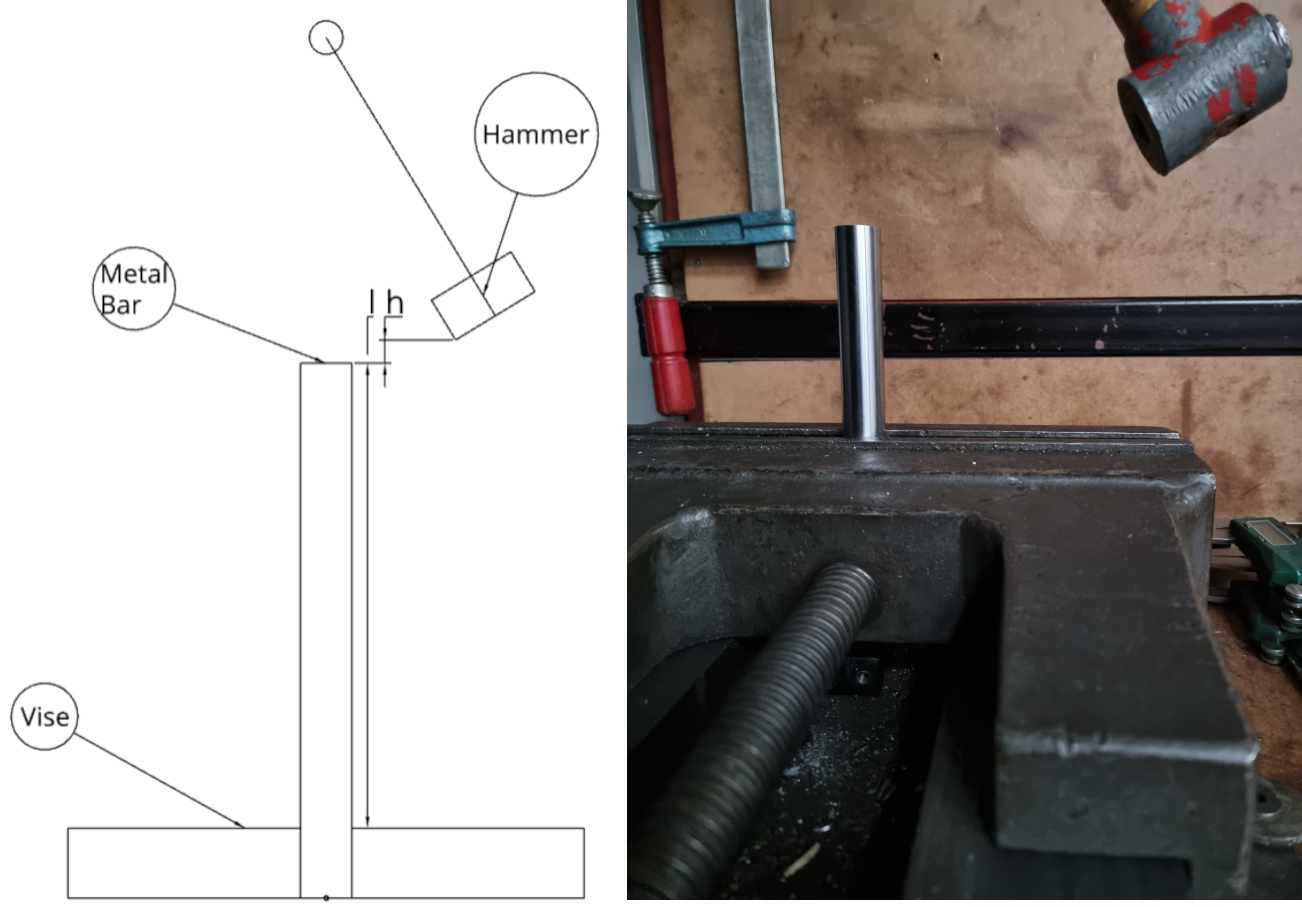
\includegraphics[width=0.8\textwidth]{setup+diag}
    \centering
    \caption{The Test Setup}\label{fig:EXPPic}
    \end{figure}
    To analyze the data, the Fast Fourier Transform was used, as explained in Section \ref{FT}, to convert the time-pressure graphs, also known as waveforms from the sound recording, such as the one seen in Figure \ref{fig:recPic} into the frequency domain, as shown in Figure \ref{fig:FFTPic}

    \begin{figure}[H]%fig:recPic
    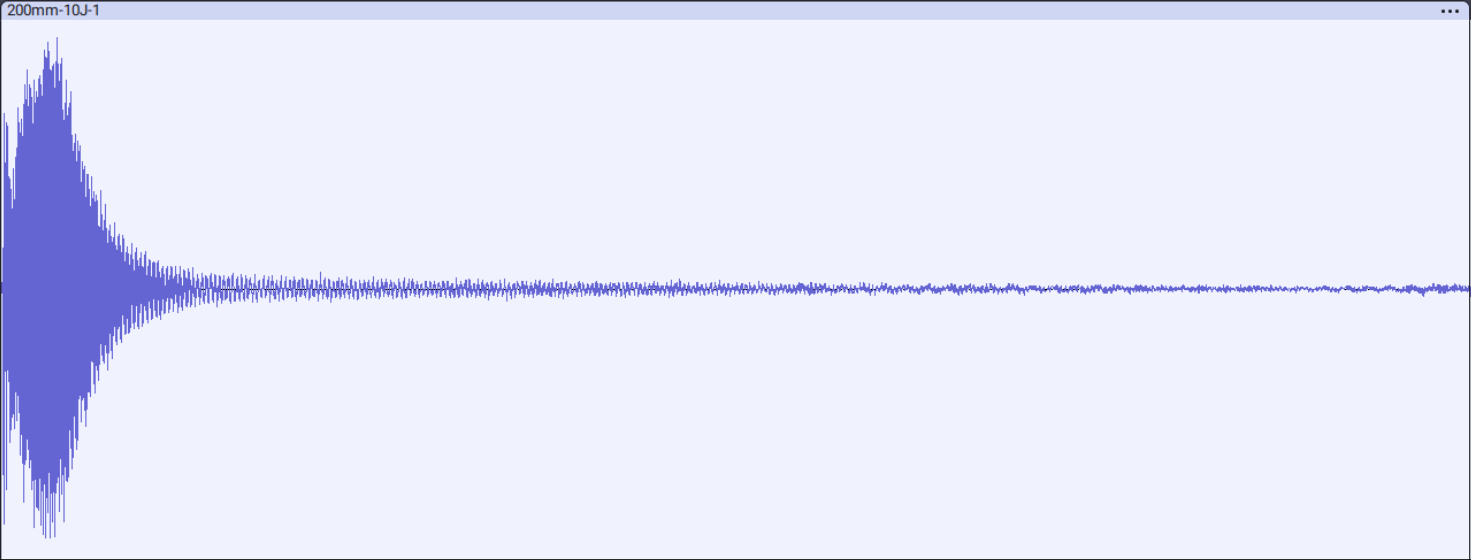
\includegraphics[width=0.9\textwidth]{Recording}
    \centering
    \caption{The Waveform From $E=10$ J and $l=200$ mm}\label{fig:recPic}
    \end{figure}
    For consistency, a 1 second section following the immediate peak(caused by the initial collision with the hammer) was taken from each recording, and that specific section was put through the FFT algorithm.\\
    \begin{figure}[H]%fig:FFPTPic
    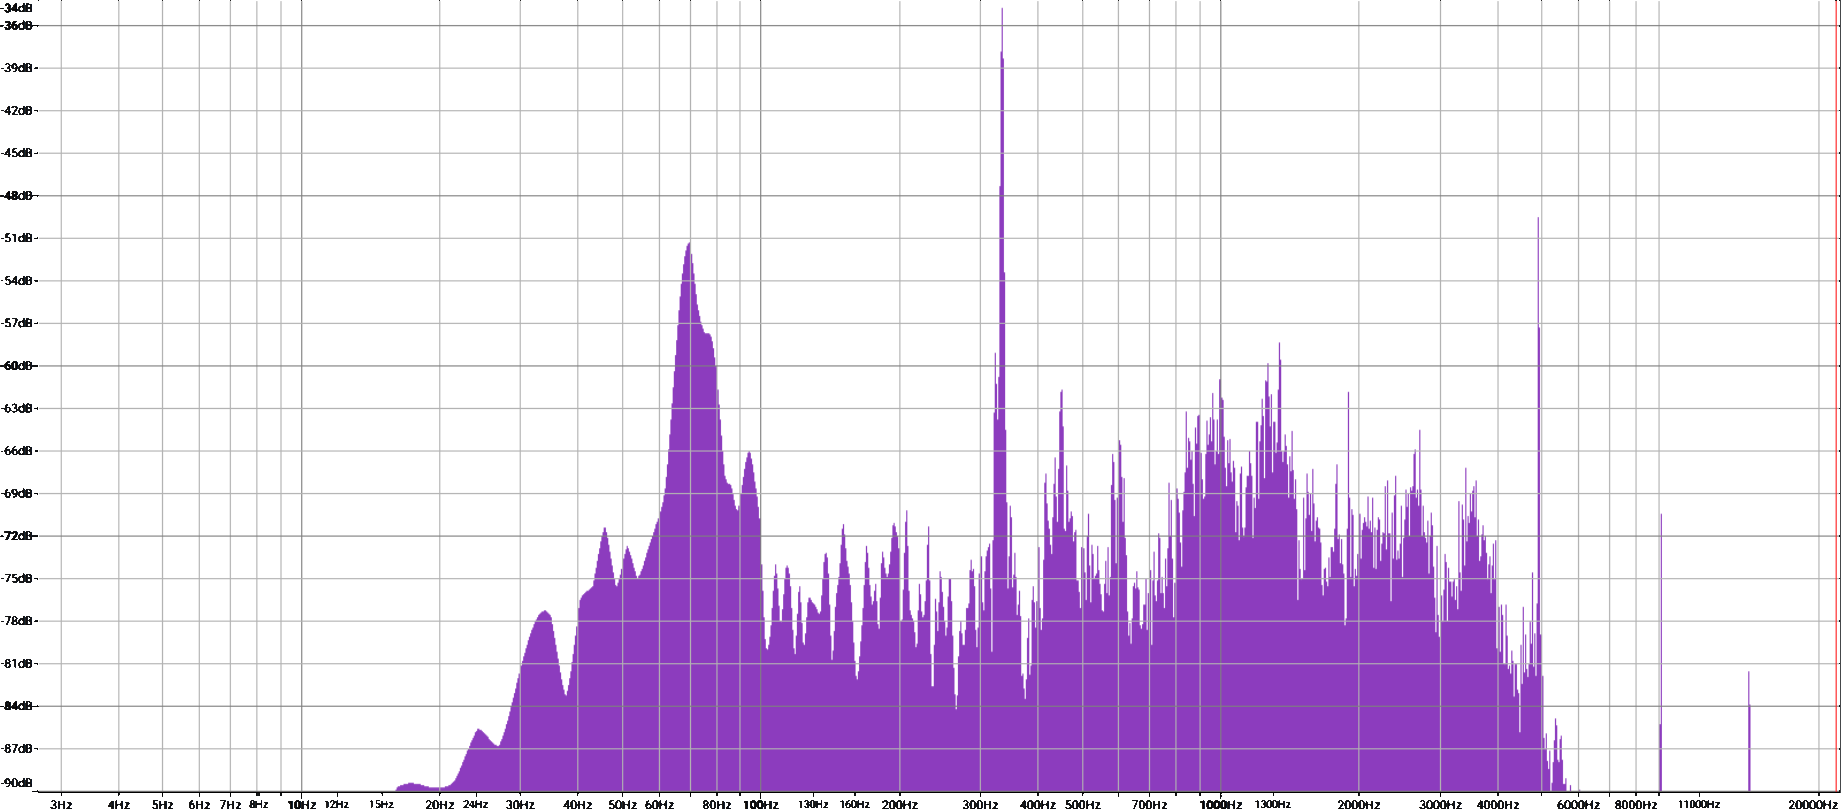
\includegraphics[width=0.8\textwidth]{FFTImage}
    \centering
    \caption{Recording Converted to Frequency Domain Using The FFT, There is a peak at 334 hz.}\label{fig:FFTPic}
    \end{figure}
    Each set of length and energy was ran 3 times to determine the magnitude of random error in the experiment. After putting every single recording through the Fast Fourier Transform algorithm and picking the peak frequency for each one, the results are seen in Figure \ref{fig:TableResults}.

    \begin{figure}[H]%fig:TableResults
    \begin{center}
    \begin{tabular}[H]{|c|c|c||c|c|c|c|}
    \hline
    $l$ & $\frac{1}{l^2}$ & $E$ & $f_1$ & $f_2$ & $f_3$ & $f_{mean}$  \\
    \hline\hline
    100mm & $10^{-4}~mm^{-2}$ & 5 J & 956 hz & 913 hz & 907 hz & $925\pm2.98$ hz \\
    \hline
    100mm & $10^{-4}~mm^{-2}$ & 7.5 J & 913 hz & 933 hz & 936 hz & $927\pm2.04$ hz \\
    \hline
    100mm & $10^{-4}~mm^{-2}$ & 10 J & 914 hz & 927 hz & 895 hz &$912\pm2.32$ hz \\
    \hline
    150mm & $10^{-4}~mm^{-2}$ & 5 J & 563 hz & 539 hz & 563 hz &$555\pm2.15$ hz \\
    \hline
    150mm & $10^{-4}~mm^{-2}$ & 7.5 J & 536 hz & 539 hz & 564 hz &$546\pm2.26$ hz \\
    \hline
    150mm & $10^{-4}~mm^{-2}$ & 10 J & 540 hz & 534 hz & 540 hz &$538\pm1.07$ hz \\
    \hline
    200mm & $10^{-4}~mm^{-2}$ & 5 J & 335 hz & 335 hz & 324 hz &$331\pm1.45$ hz \\
    \hline
    200mm & $10^{-4}~mm^{-2}$ & 7.5 J & 335 hz & 334 hz & 334 hz &$334\pm0.44$ hz \\
    \hline
    200mm & $10^{-4}~mm^{-2}$ & 10 J & 334 hz & 334 hz & 332 hz &$333\pm0.62$ hz \\
    \hline
    \end{tabular}
    \end{center}
    \caption{The Results Of the Experiment}\label{fig:TableResults}
    \end{figure}
    Looking at Figure \ref{fig:TableResults}, It is clear that $E$ and $f$ have no relation, as suggested in \eqref{eqn:theory} and simulated in Section \ref{FEA}, with this, every subsequent section will only take recordings where $E=10$ J into account.

    In a similar manner to Figure \ref{fig:regression}, the data in Figure \ref{fig:TableResults} has been graphed and a linear fit line has been calculated, and shown in Figure \ref{fig:EXPregression}.

    \begin{figure}[H]%fig:EXPregerssion
    \begin{center}
    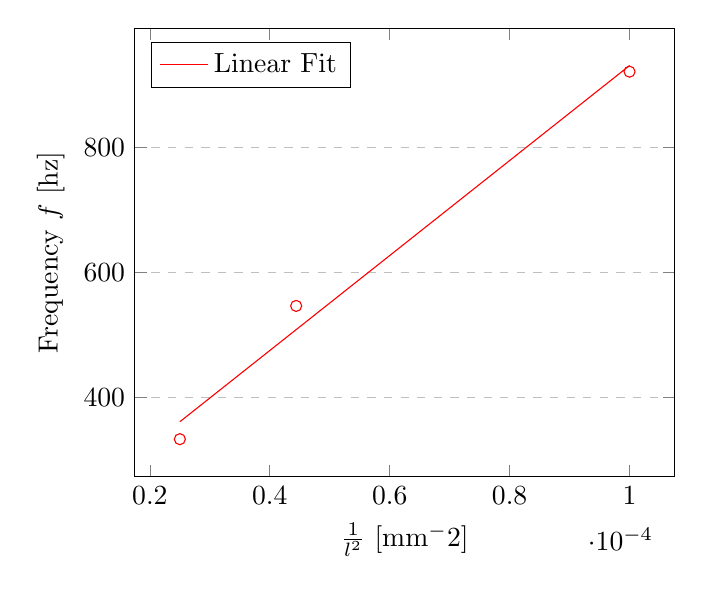
\begin{tikzpicture}
    \begin{axis}[
        xlabel={$\frac{1}{l^{2}}$ [mm$^-2$]},
        ylabel={Frequency $f$ [hz]},
        legend pos=north west,
        ymajorgrids=true,
        grid style=dashed,
    ]
    \addplot [
        domain=2.5e-5:1e-4,
        samples=100,
        color=red,
        ]
        {7605636.67232598*x + 170.755};
    \addlegendentry{Linear Fit}
    \addplot+[
        only marks,
        color=red,
        mark=o,
        ]
        coordinates {
        (1e-4,921.56)(4.44e-5,546.44)(2.5e-5,333)
        };
    \end{axis}
    \end{tikzpicture}

    \caption{Table of ($\frac{1}{l^{2}}$,$f$) and linear regression}\label{fig:EXPregression}
    \end{center}
    \end{figure}
    From the analysis, the values $R^2=0.97809$ showing strong correlation and $f=7605636\frac{1}{l^{2}}+170$ were acquired, or transformed to $f\propto\frac{1}{l^{2}}+2.2\times10^{-5}$\\
    While the result is once again, off by $2.2\times10^{-5}$, it is small enough to be negligible.

\section{Results And Analysis}\label{ResultsAnalysis}%500
    \subsection{Uncertainty Analysis}
\section{Discussion}%500
\section{Conclusion}%500

\pagebreak
\addcontentsline{toc}{section}{References}
\printbibliography


\end{document}

